\maketitle
\tableofcontents
\newpage

\section{Zielsetzung}
Ziel des Versuches ist es, die \textbf{Leerlaufspannung} und den \textbf{\textbf{Innenwiderstand}}
verschiedener Spannungsquellen zu ermitteln.
\section{Theorie}
Die \textbf{Leerlaufspannung} $U_0$ ist die Spannung, die gemessen wird, wenn kein Strom fließt.
Sie wird direkt an den Klemmen der Spannungsquelle abgenommen. Wenn über einen Verbraucher
mit Lastwiderstand $R_a$ ein endlicher Strom $I$ fließt, dann gilt für die nun gemessene
"Klemmenspannung" $U_k$, die ebenfalls an den Klemmen der Spannungsquelle abgenommen wird,
\begin{equation*}
    U_k < U_0 \ .
\end{equation*}
Mit dem zweiten Kirchoffschen Gesetz
\begin{equation}
  \sum_n U_{0_n} = \sum_m R_m \, I_m
  \label{eqn:4}
\end{equation}
folgt für die betrachtete Situation
\begin{equation}
    U_0 = I \, R_i + I \, R_a \ .
    \label{eqn:5}
\end{equation}
\begin{figure}[h]
  \centering
  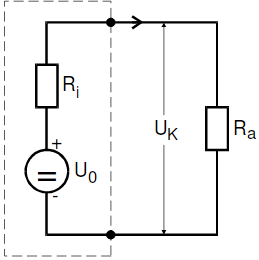
\includegraphics[scale=0.7]{theorie.png}
  \caption{Schaltbild einer idealen Spannungsquelle mit Außenwiderstand $R_i$ und
  Lastwiderstand $R_a$.}
  \label{fig:1}
\end{figure}
Dabei ist $R_i$ der \textbf{\textbf{Innenwiderstand}} der Spannungsquelle. Die Klemmenspannung
$U_k$, siehe \ref{fig:1}, lässt sich somit bestimmen aus \eqref{eqn:5}
\begin{equation}
    U_k = I \, R_a = U_0 - I \, R_i \ .
    \label{eqn:6}
\end{equation}
Damit ist auch die Beziehung
\begin{equation*}
    U_k \approx U_0
\end{equation*}
für die \textbf{Leerlaufspannung} gezeigt, da für diesen Fall in \eqref{eqn:6}
$I$ vernachlässigbar klein wird. Für diese Betrachtungsweise ist die Spannungsquelle
eine sogenannte ideale Spannungsquelle mit einem \textbf{Innenwiderstand} von 0 und einem in
Reihe geschalteten Außenwiderstand $R_i$, der den \textbf{Innenwiderstand} simuliert.

Bei einem RC-Generator wird durch die Änderung des Belastungsstroms das elektrische
Verhalten der Quelle festgelegt. In diesem Fall ist der \textbf{Innenwiderstand} eine differentielle
Größe mit
\begin{equation}
  R_i = \frac{\symup dU_k}{\symup d I} \ .
  \label{eqn:7}
\end{equation}

Für eine Schaltung mit einer Gegenspannung größer als $U_0$\footnote{siehe Kapitel \ref{sec:3.2}} gilt
\begin{equation}
    U_k = U_0 + R_i \, I
    \label{eqn:8}
\end{equation}

\section{Durchführung}
\subsection{Versuchsaufbau}
\begin{figure}
  \centering
  \begin{subfigure}{0.45\textwidth}
    \centering
    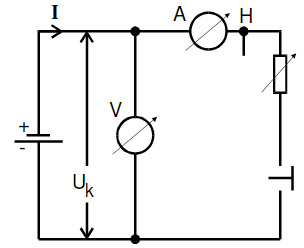
\includegraphics[scale=0.6]{durch.png}
    \caption{Schaltbild zur Messung von $U_k$ in Abhängigkeit von $I$.}
    \label{sub:1}
    \qquad
  \end{subfigure}
  \begin{subfigure}{0.45\textwidth}
    \centering
    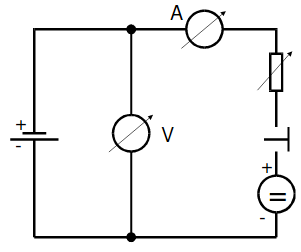
\includegraphics[scale=0.6]{durch2.png}
    \caption{Schaltbild zur Messung von $U_k$ in Abhängigkeit von $I$ mit Gegenspannung.}
    \label{sub:2}
    \qquad
  \end{subfigure}
  \caption{Schaltbilder zu Aufgabe 2 (\ref{sub:1}) und Aufgabe 3 (\ref{sub:2})
  der Versuchsdurchführung.}
  \label{fig:2}
\end{figure}
\subsection{Versuchsdurchführung}
\label{sec:3.2}
Als erstes wurde die \textbf{Leerlaufspannung} einer Monozelle mit einem Spannungsmesser
und der Eingangswiderstand $R_v$ bestimmt. Danach wurde mit der Schaltung in \ref{sub:1}
die Klemmspannung $U_k$ in Abhängigkeit von $I$ gemessen. Der Variationsbereich des
Belastungswiderstandes $R_a$ liegt zwischen 0 und $\SI{50}{\ohm}$. % Schrittweite angegeben

Als nächstes wurde die Schaltung \ref{sub:2} aufgebaut und die Messung wiederholt.
Dabei ist die Gegenspannung $\SI{2}{\volt}$ größer als die der Monozelle und der
Stromfluss kehrt sich um.

Als letzes wird die Monozelle durch eine Rechteck- und eine Sinusspannung, die
durch einen RC-Generator erzeugt werden, ausgetauscht. Die Variationsbereiche der
Belastungswiderstände lauten:
\begin{itemize}
  \item Sinusspannung: 20 $\leq$ $R_a$ $\le$ $\SI{250}{\ohm}$
  \item Rechteckspannung: 0,1 $\leq$ $R_a$ $\leq$ $\SI{5}{\kilo\ohm}$
\end{itemize}
Die Frequenzen lauten % Frequenzen einfügen
 \section{Fehlerrechnung}
 Es gibt:
 \begin{equation}
   \bar{T} = \frac{1}{n} \sum_{i=1}^{n} T_{i}
   \label{eqn:1}
 \end{equation}
 den Mittelwert und:
 \begin{equation}
   \sigma_{\bar{T}} = \sqrt{\frac{1}{n(n-1)} \sum_{i=1}^{n}(\bar{T}-T_i)^2}
   \label{eqn:2}
 \end{equation}
 den Fehler des Mittelwertes. Falls zwei fehlerbehaftete Größen in einer Gleichung
 zur Bestimmung einer anderen Größe Verwendung finden, dann berechnte sich der Gesamtfehler
 nach der Gaußschen Fehlerfortpflanzung zu
 \begin{equation}
     \symup \Delta f(x_1, x_2, ..., x_n) = \sqrt{\left(\frac{\symup df}{\symup dx_1} \symup \Delta
     x_1 \right)^2 +    \left(\frac{\symup df}{\symup dx_2} \symup \Delta
     x_2 \right)^2 + ... + \left(\frac{\symup df}{\symup dx_n} \symup \Delta x_n \right)^2} \ .
     \label{eqn:3}
 \end{equation}

\section{Auswertung}

\section{Diskussion}

\newpage
\nocite{*}
\printbibliography
